\section{RISMC Approach to PRA}
\label{sec:rismc}
The RISMC approach~\cite{RISMC} employs both deterministic and stochastic methods 
in a single analysis framework (see Figure~\ref{fig:RISMCoverview}). In the deterministic method 
set we include:
\begin{itemize}
  \item Modeling of the thermal-hydraulic behavior of the plant~\cite{BWR_SBO_Mandelli,BWRanalysis}
  \item Modeling of external events such as flooding~\cite{mandelliPSA2015}
  \item Modeling of the operators’ responses to the accident scenario~\cite{HRA_BoringReport2014}
\end{itemize}

\begin{figure}
    \centering
    \centerline{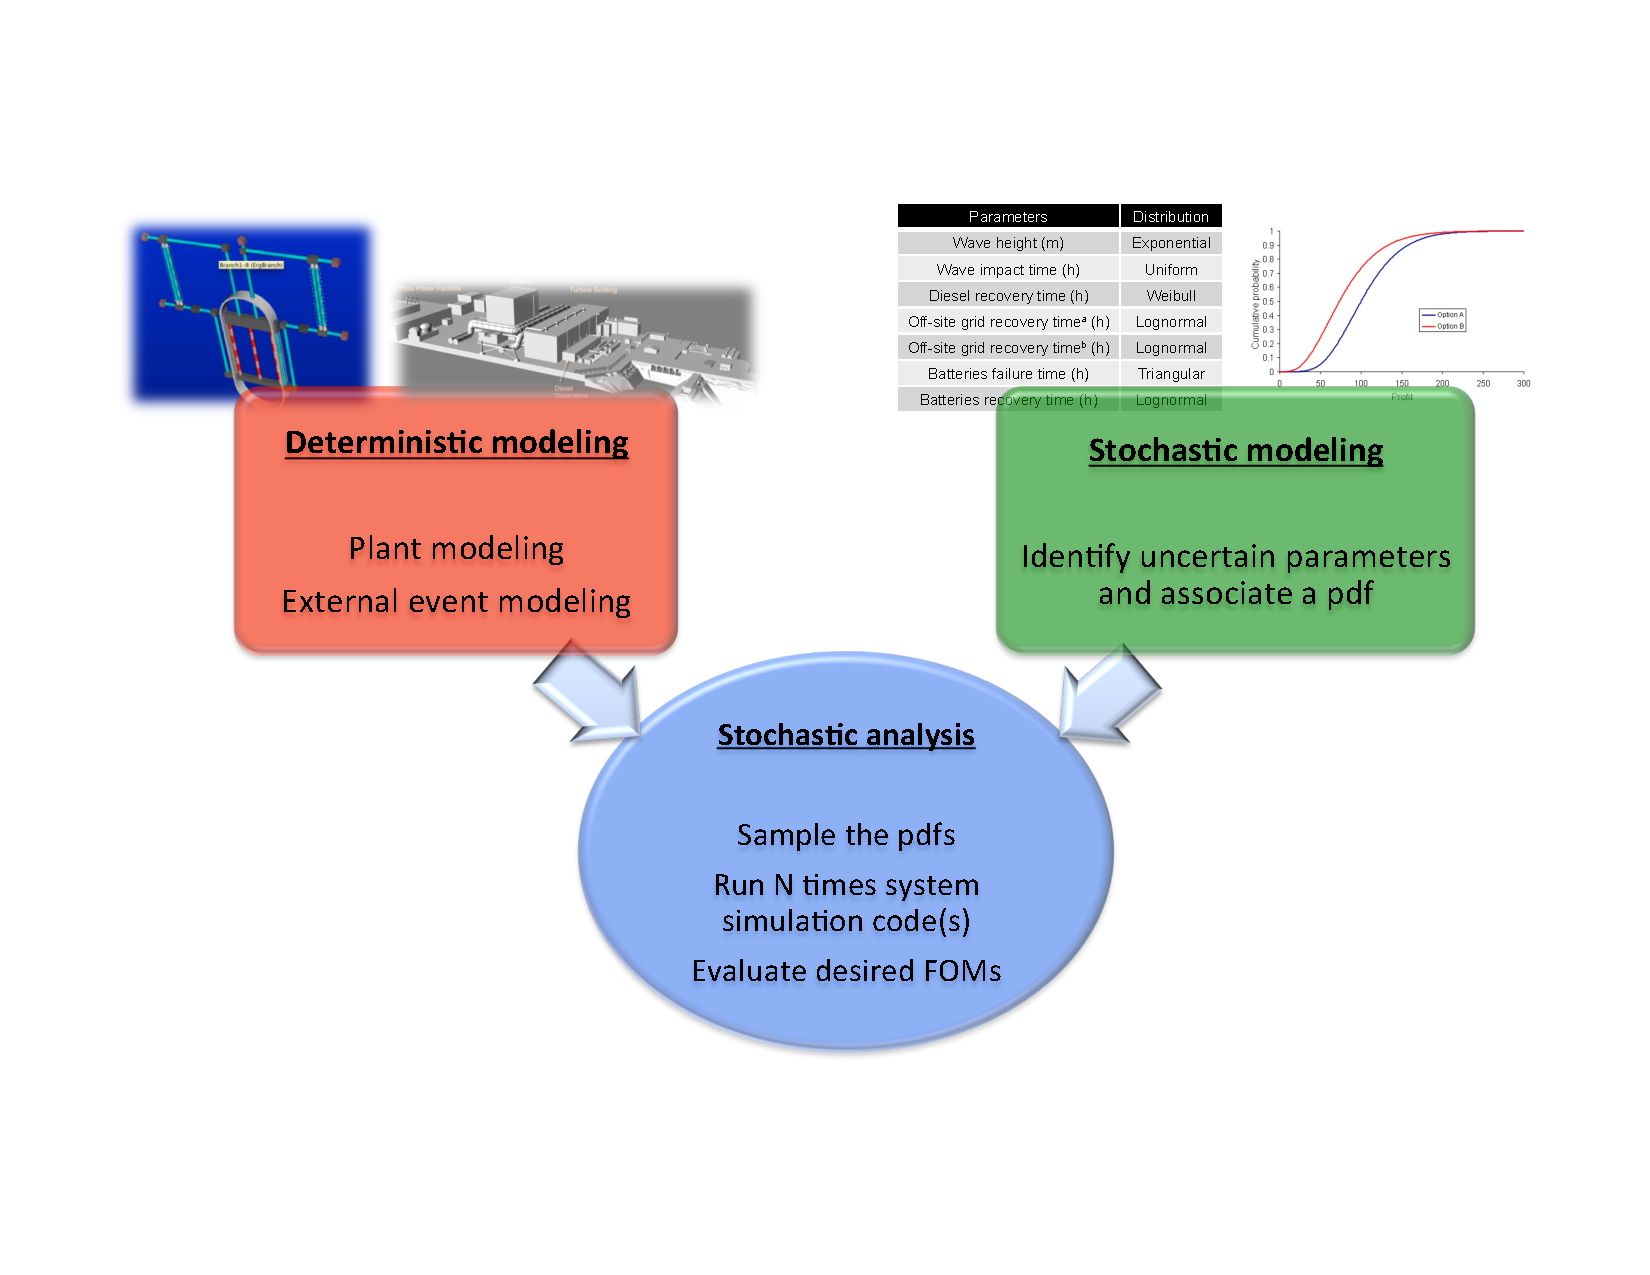
\includegraphics[scale=0.4]{RISMCoverview.pdf}}
    \caption{Overview of the RISMC approach}
    \label{fig:RISMCoverview}
\end{figure}

Note that deterministic modeling of the plant or external events can be performed by employing specific 
simulator codes but also surrogate models~\cite{ROM}, known as reduced order models (ROM). ROMs would be employed 
in order to decrease the high computational costs of employed codes. In addition, multi-fidelity codes 
can be employed to model the same system; the idea is to switch from low-fidelity to high-fidelity code 
when higher accuracy is needed (e.g., use low-fidelity codes for steady-state conditions and high-fidelity 
code for transient conditions)

In the stochastic modeling we include all stochastic parameters that are of interest in the PRA analysis 
such as uncertain parameters and stochastic failure of system/components.
As mentioned earlier, the RISMC approach heavily relies on multi-physics system simulator codes 
(e.g., RELAP5-3D~\cite{relap5}) coupled with stochastic analysis tools (e.g., RAVEN~\cite{raven}).  
From a PRA point of view, this type of simulation can be described by using two sets of variables:
\begin{itemize}
  \item $\boldsymbol c = \boldsymbol c(t)$ represents the status of components and systems of the simulator 
        (e.g., status of emergency core cooling system, AC system)
  \item $\boldsymbol \theta = \boldsymbol \theta (t)$ represents the temporal evolution of a simulated 
        accident scenario, i.e., $\boldsymbol \theta (t)$ represents a single simulation run. 
        Each element of $\boldsymbol \theta$ can be for example the values of temperature or pressure in 
        a specific node of the simulator nodalization.
\end{itemize}

From a mathematical point of view, a single simulator run can be represented as a single trajectory in the 
phase space. The evolution of such a trajectory in the phase space can be described as follows:
\begin{equation}
  \begin{cases}
    \dfrac{\partial \boldsymbol \theta }{\partial t}  = \boldsymbol \Xi (\boldsymbol \theta , \boldsymbol c, \boldsymbol s , t)   \\ \\ 
    \dfrac{\partial \boldsymbol c }{\partial t}  = \boldsymbol \Gamma (\boldsymbol \theta , \boldsymbol c, \boldsymbol s , t) 
  \end{cases}    
  \label{eq:trajectory}
\end{equation}
where:
\begin{itemize}
  \item $\boldsymbol \Xi$ is the actual simulator code that describes how θ evolves in time
  \item $\boldsymbol \Gamma$ is the operator which describes how c evolves in time , i.e., the status 
        of components and systems at each time step
  \item $\boldsymbol C$ is the set of stochastic parameters.
\end{itemize}

Starting from the system located in an initial state, $\boldsymbol \theta (t=0) = \boldsymbol \theta(0)$, 
and the set of stochastic parameters (which are generally generated through a stochastic sampling process), 
the simulator determine at each 
time step the temporal evolution of $\boldsymbol \theta (t)$. At the same time, the system control logic  determines the status 
of the system and components $\boldsymbol c(t)$.
 
By using the RISMC approach, the PRA analysis is performed by []:
\begin{enumerate}
  \item Associating a probabilistic distribution function (pdf) to the set of parameters $\boldsymbol s$ (e.g., timing of events)
  \item Performing stochastic sampling of the pdfs defined in Step 1
  \item Performing a simulation run given $\boldsymbol s$ sampled in Step 2, i.e., solve the system of equations~\ref{??}
\end{enumerate}

Repeating Steps 2 and 3 $M$ times and evaluating user defined stochastic parameters such as core damage (CD) 
probability ($P_{CD}$).
